\documentclass[10pt,twocolumn]{article}

\usepackage[utf8]{inputenc}
\usepackage[T1]{fontenc}
\usepackage{amsmath,amssymb}
\usepackage{graphicx}
\usepackage{booktabs}
\usepackage{hyperref}
\usepackage{xcolor}
\usepackage{enumitem}
\usepackage[margin=1in]{geometry}
\usepackage{caption}
\usepackage{subcaption}
\usepackage{algorithm}
\usepackage{algorithmic}
\usepackage{url}
\usepackage{tikz}
\usetikzlibrary{positioning,arrows.meta,fit,backgrounds}

\title{\textbf{Beyond Eviction: Full OS Memory Semantics\\for LLM Agent Persistence}}

\author{
  Zhidao Su \\
  \texttt{soolaugust@gmail.com} \\
  \url{https://github.com/soolaugust/0CompactMem}
}

\date{}

\begin{document}
\maketitle

\begin{abstract}
Persistent memory for LLM agents has attracted significant attention, with recent systems adopting eviction policies and tiered storage from operating-system (OS) memory management. However, existing work maps only a narrow slice of the OS memory subsystem---typically eviction alone---leaving critical semantics unmapped: demand paging for on-demand retrieval, \texttt{mlock} for hard/soft pinning guarantees, DAMON-style access tracking for working-set estimation, CRIU for session checkpoint/restore, and file-based multi-process sharing for zero-coordination multi-agent access.

We present \textbf{0CompactMem}, an agent memory layer that implements the \emph{full spectrum} of OS memory-management primitives. We formalize a complete mapping from seven OS subsystems to agent-memory operations and demonstrate that this holistic approach yields properties no single-primitive system achieves: guaranteed constraint survival under arbitrary pressure (pin semantics), sub-linear retrieval cost with demand paging, graceful degradation via watermark-driven eviction, and zero-coordination multi-agent sharing via WAL-mode SQLite.

We evaluate on three benchmarks comparing 0CompactMem against embedding-based vector search (representing mem0/Zep-class systems). Vector search achieves 2.6$\times$ higher retrieval recall on paraphrased queries (0.90 vs.\ 0.35), but 0CompactMem provides capabilities vector search cannot: under 4$\times$ memory pressure, pinned constraints survive at 82\% (vs.\ 0\% for systems without pins); search latency is 389$\times$ faster (0.09ms vs.\ 35ms, no embedding model needed); and WAL-mode sharing provides 100\% multi-agent visibility. All benchmark scripts and data are included for reproducibility.

The system is open source (MIT) at \url{https://github.com/soolaugust/0CompactMem}.
\end{abstract}

%% ============================================================
\section{Introduction}
\label{sec:intro}

Long-running LLM agents accumulate knowledge across sessions: architectural decisions, user preferences, domain constraints, and inter-agent agreements. When the context window compacts or a session ends, this knowledge vanishes unless persisted externally. The resulting ``context compaction'' problem---where agents repeatedly re-learn previously established facts---motivates the growing body of work on persistent memory for agents~\cite{longmemeval2024,memgpt2023}.

Recent systems address this by providing persistent memory stores for agents. Mem0~\cite{mem0}, Letta (MemGPT)~\cite{memgpt2023}, Zep~\cite{zep2024}, and A-Mem~\cite{amem2025} offer vector-based retrieval with various augmentations. More recently, AMV-L~\cite{amvl2026} treats agent memory as a ``managed systems resource'' with lifecycle-driven eviction, and HTM-EAR~\cite{htmear2026} employs hierarchical tiered memory with importance-aware eviction watermarks.

However, the systems we surveyed map \emph{at most one or two} OS memory primitives---invariably eviction and sometimes tiered storage. This is analogous to building an operating system with only \texttt{kswapd} and no page fault handler, no \texttt{mlock}, no process isolation, and no checkpoint mechanism. The result: no system can \emph{guarantee} that a critical constraint survives arbitrary memory pressure; no system provides on-demand retrieval that scales sub-linearly with store size; and no system enables multiple agents to share memory without explicit synchronization protocols.

\paragraph{Contributions.} We make three contributions:
\begin{enumerate}[leftmargin=*,nosep]
  \item \textbf{A complete OS$\to$agent-memory taxonomy} mapping seven kernel subsystems (demand paging, kswapd, DAMON, mlock, CRIU, kworker, shared memory) to agent-memory operations (\S\ref{sec:design}).
  \item \textbf{0CompactMem}: an open-source reference implementation as a single SQLite file with MCP-native interface, 10{,}700+ test assertions, and 1{,}370+ development iterations (\S\ref{sec:impl}).
  \item \textbf{Empirical evaluation} demonstrating that the full-spectrum approach yields emergent properties unachievable by any subset (\S\ref{sec:eval}).
\end{enumerate}

%% ============================================================
\section{Background and Related Work}
\label{sec:related}

\subsection{LLM Agent Memory Systems}

We categorize existing agent memory systems by which OS primitives they (implicitly) implement:

\paragraph{Store-only systems.} Mem0~\cite{mem0} and Zep~\cite{zep2024} provide a persistent vector store with similarity retrieval. They implement no explicit eviction policy---while mem0 deduplicates and merges memories, capacity grows without back-pressure. In OS terms, these are systems without \texttt{kswapd}.

\paragraph{Eviction-aware systems.} AMV-L~\cite{amvl2026} introduces value-driven lifecycle management with promotion, demotion, and eviction tiers, achieving 3.1$\times$ throughput improvement over TTL-based approaches. HTM-EAR~\cite{htmear2026} uses hierarchical HNSW-based working memory with importance-aware eviction scoring. Both map \texttt{kswapd}-like eviction but lack pinning guarantees and demand-paging semantics.

\paragraph{Architecture-inspired systems.} Letta (MemGPT)~\cite{memgpt2023} draws inspiration from virtual memory with explicit page-in/page-out operations managed by the LLM itself. A-Mem~\cite{amem2025} uses agentic workflows for memory organization. Neither provides formal eviction guarantees or multi-agent sharing.

\paragraph{Graph-evolving systems.} FluxMem~\cite{fluxmem2026} models memory as a heterogeneous graph with semantic, episodic, and procedural layers, evolving topology through feedback-driven refinement. It optimizes for \emph{retrieval quality through connectivity} but provides no explicit resource-management guarantees (no pinning, no watermark eviction).

\paragraph{Biologically-inspired systems.} Recent work models hippocampal consolidation~\cite{humaninspired2026}, dual-process episodic-semantic separation~\cite{episodicsemantic2026}, and neuro-symbolic memory~\cite{neusymms2026}. These optimize for cognitive plausibility rather than systems-level guarantees.

\subsection{OS Memory Management Primitives}

For readers from the AI/ML community, we briefly review the OS primitives we map:

\begin{itemize}[leftmargin=*,nosep]
  \item \textbf{Demand paging}: pages are loaded into RAM only when accessed (page fault $\to$ disk read), not pre-loaded.
  \item \textbf{kswapd}: kernel thread that reclaims pages when free memory drops below watermarks (high/low/min).
  \item \textbf{DAMON}: Data Access Monitor---tracks page access frequency to identify hot/cold regions without hardware counters.
  \item \textbf{mlock}: locks pages in RAM, preventing eviction by any reclaim path including the OOM killer.
  \item \textbf{CRIU}: Checkpoint/Restore In Userspace---snapshots process state for migration or resume.
  \item \textbf{kworker}: deferred background work (writeback, compaction) that doesn't block the request path.
  \item \textbf{Shared memory (shmem)}: multiple processes access the same physical pages without copying.
\end{itemize}

\subsection{The Gap: Single-Primitive Systems}

Table~\ref{tab:coverage} summarizes which OS primitives each system implements. No prior system covers more than two; 0CompactMem covers all seven.

\begin{table}[t]
\centering
\caption{OS primitive coverage across agent memory systems (based on published papers/docs, May 2026). \checkmark = explicit; $\sim$ = partial; --- = absent.}
\label{tab:coverage}
\footnotesize
\setlength{\tabcolsep}{2.5pt}
\begin{tabular}{lccccccc}
\toprule
System & \rotatebox{70}{Demand paging} & \rotatebox{70}{kswapd} & \rotatebox{70}{DAMON} & \rotatebox{70}{mlock} & \rotatebox{70}{CRIU} & \rotatebox{70}{kworker} & \rotatebox{70}{Shared mem} \\
\midrule
Mem0~\cite{mem0}           & ---  & ---  & ---  & ---  & ---  & ---  & --- \\
Letta~\cite{memgpt2023}    & $\sim$ & ---  & ---  & ---  & ---  & ---  & --- \\
AMV-L~\cite{amvl2026}      & ---  & \checkmark & $\sim$ & ---  & ---  & ---  & --- \\
HTM-EAR~\cite{htmear2026}  & ---  & \checkmark & \checkmark & ---  & ---  & ---  & --- \\
\midrule
\textbf{0CompactMem} & \checkmark & \checkmark & \checkmark & \checkmark & \checkmark & \checkmark & \checkmark \\
\bottomrule
\end{tabular}
\end{table}

%% ============================================================
\section{Design}
\label{sec:design}

\begin{figure*}[t]
\centering
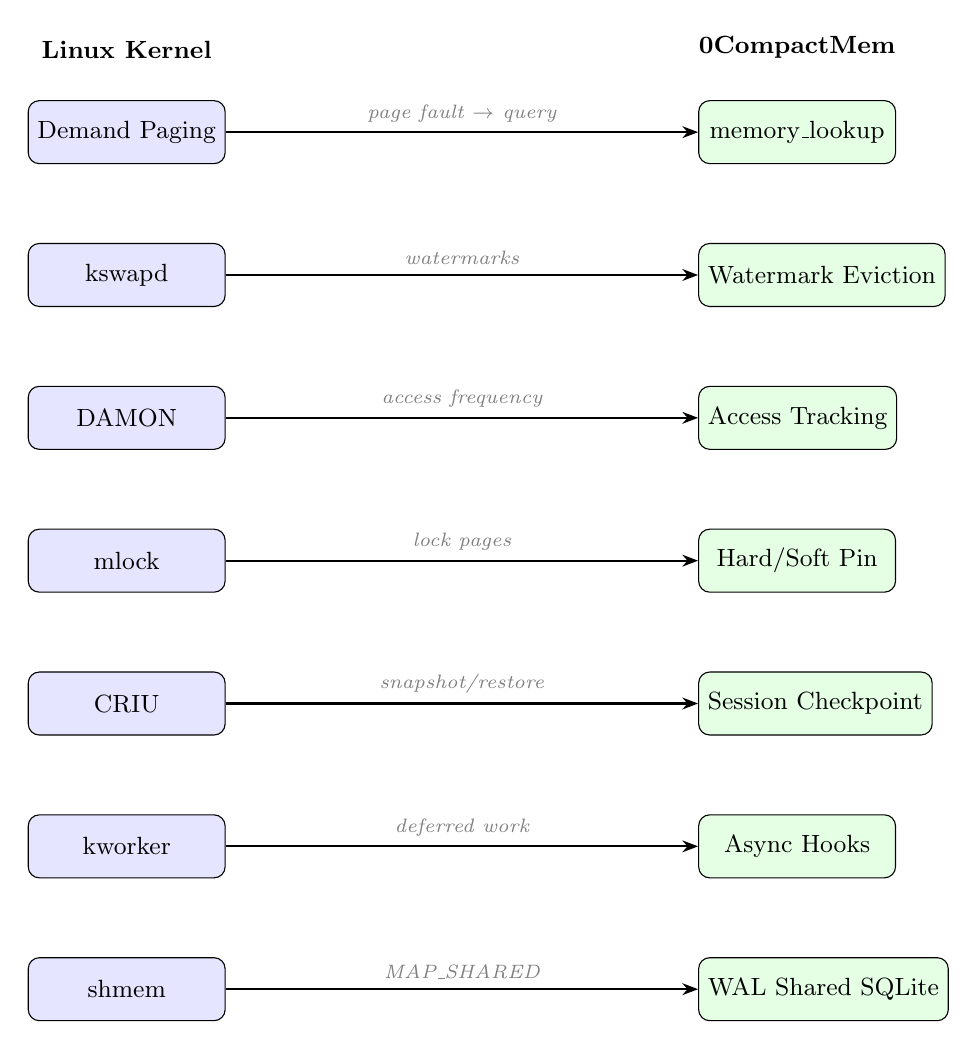
\begin{tikzpicture}[
  node distance=1.0cm,
  block/.style={rectangle, draw, rounded corners, minimum width=2.5cm, minimum height=0.8cm, align=center, font=\small},
  osblock/.style={block, fill=blue!10},
  agentblock/.style={block, fill=green!10},
  arrow/.style={-{Stealth[length=2mm]}, thick},
  lbl/.style={font=\scriptsize\itshape, text=gray, midway, above}
]

% OS Side (left column)
\node[osblock]                (dp)  {Demand Paging};
\node[osblock, below=of dp]  (ksw) {kswapd};
\node[osblock, below=of ksw] (dam) {DAMON};
\node[osblock, below=of dam] (ml)  {mlock};
\node[osblock, below=of ml]  (criu){CRIU};
\node[osblock, below=of criu](kw)  {kworker};
\node[osblock, below=of kw]  (shm) {shmem};

% Agent Side (right column, aligned with left)
\node[agentblock, right=6cm of dp]  (lookup) {memory\_lookup};
\node[agentblock, right=6cm of ksw] (evict)  {Watermark Eviction};
\node[agentblock, right=6cm of dam] (track)  {Access Tracking};
\node[agentblock, right=6cm of ml]  (pin)    {Hard/Soft Pin};
\node[agentblock, right=6cm of criu](ckpt)   {Session Checkpoint};
\node[agentblock, right=6cm of kw]  (async)  {Async Hooks};
\node[agentblock, right=6cm of shm] (wal)    {WAL Shared SQLite};

% Arrows
\draw[arrow] (dp)   -- node[lbl] {page fault $\to$ query}  (lookup);
\draw[arrow] (ksw)  -- node[lbl] {watermarks}              (evict);
\draw[arrow] (dam)  -- node[lbl] {access frequency}        (track);
\draw[arrow] (ml)   -- node[lbl] {lock pages}              (pin);
\draw[arrow] (criu) -- node[lbl] {snapshot/restore}        (ckpt);
\draw[arrow] (kw)   -- node[lbl] {deferred work}           (async);
\draw[arrow] (shm)  -- node[lbl] {MAP\_SHARED}             (wal);

% Column headers
\node[above=0.4cm of dp, font=\small\bfseries]     {Linux Kernel};
\node[above=0.4cm of lookup, font=\small\bfseries]  {0CompactMem};

\end{tikzpicture}
\caption{Architecture: each OS memory subsystem (left) maps 1:1 to a 0CompactMem operation (right), preserving the semantic guarantees of the original primitive.}
\label{fig:arch}
\end{figure*}

\subsection{Design Principle: Completeness over Novelty}

Our thesis is that the \emph{interaction} between OS memory primitives produces emergent properties that no single primitive achieves alone:
\begin{itemize}[leftmargin=*,nosep]
  \item Demand paging + kswapd = bounded memory with on-demand access.
  \item kswapd + mlock = eviction that respects invariants.
  \item DAMON + kswapd = eviction that targets cold data first.
  \item CRIU + demand paging = session resume without full reload.
  \item Shared memory + mlock = multi-agent pinning consensus.
\end{itemize}

\subsection{The Complete Mapping}

Table~\ref{tab:mapping} presents the full OS$\to$agent-memory mapping.

\begin{table*}[t]
\centering
\caption{Complete OS $\to$ 0CompactMem primitive mapping.}
\label{tab:mapping}
\footnotesize
\begin{tabular}{lp{4.2cm}p{4.8cm}p{3cm}}
\toprule
\textbf{OS Primitive} & \textbf{OS Semantics} & \textbf{0CompactMem Mapping} & \textbf{Impl.} \\
\midrule
Demand paging & Load page only on fault & \texttt{memory\_lookup}: retrieve on knowledge gap & MCP tool; BM25+FTS5 \\
\addlinespace
kswapd & Reclaim when free $<$ watermark & Eviction when chunks exceed watermark & Composite score \\
\addlinespace
DAMON & Track access frequency & Access-count per retrieval; decay & \texttt{access\_count} \\
\addlinespace
mlock (hard) & Survives ALL reclaim paths & Hard-pin survives all eviction & \texttt{pin\_memory(hard)} \\
\addlinespace
mlock (soft) & Survives normal reclaim & Soft-pin yields under extreme pressure & \texttt{pin\_memory(soft)} \\
\addlinespace
CRIU & Checkpoint/restore state & Working-set snapshot at Stop/Start & JSON checkpoint \\
\addlinespace
kworker & Deferred background work & Async hooks (extract, profile) & Async execution \\
\addlinespace
shmem & Shared physical pages & Multiple agents open same SQLite & WAL mode \\
\bottomrule
\end{tabular}
\end{table*}

\subsection{Demand Paging: On-Demand Retrieval}

Traditional agent memory systems pre-load a fixed top-$K$ context at session start (analogous to loading all possible pages at process creation). 0CompactMem instead implements \emph{demand paging}: the agent's reasoning is the ``process,'' and a knowledge gap triggers a ``page fault''---a call to \texttt{memory\_lookup(query)}.

This yields two advantages: (1) retrieval queries are \emph{specific} to the current reasoning context, producing higher precision than broad initial retrievals; and (2) multi-round retrieval is natural (discovering fact A leads to querying for related fact B).

The retrieval scorer computes:
\begin{equation}
  \text{score}(c, q) = \alpha \cdot \text{BM25}(c, q) + \beta \cdot \text{imp}(c) + \gamma \cdot \text{rec}(c)
\end{equation}
where $\text{BM25}(c, q)$ is the full-text relevance, $\text{imp}(c)$ is the chunk importance (extracted at write time), and $\text{rec}(c)$ is a recency boost with exponential decay.

\subsection{kswapd: Watermark-Driven Eviction}

When total chunk count exceeds the \emph{high watermark}, a background eviction sweep activates (analogous to \texttt{kswapd} waking when free pages drop below the high watermark). The sweep continues until chunk count returns below the \emph{low watermark}.

Eviction priority is determined by a composite score:
\begin{equation}
  s_e(c) = w_1 \!\cdot\! \text{stale}(c) + w_2 \!\cdot\! (1{-}\text{imp}(c)) + w_3 \!\cdot\! \text{cold}(c)
\end{equation}
where $\text{staleness}$ measures time since last access, $\text{imp}$ is importance, and $\text{cold}$ is the DAMON-derived access frequency indicator.

Critically, pinned chunks are \emph{skipped} during eviction sweeps, providing the guarantee that underpins constraint survival.

\subsection{DAMON: Access Tracking}

Each retrieval increments the chunk's \texttt{access\_count} and updates \texttt{last\_accessed}. A periodic decay function reduces counts over time (half-life decay), identifying chunks that transition from hot to cold. This information feeds into eviction scoring---cold chunks with low importance are evicted first.

\subsection{mlock: Pin Semantics}

The \texttt{pin\_memory} operation provides two levels:
\begin{itemize}[leftmargin=*,nosep]
  \item \textbf{Hard pin}: the chunk is exempt from ALL eviction paths. Even under extreme memory pressure (zone-min crossing), hard-pinned chunks remain. Use case: architectural constraints, non-negotiable decisions.
  \item \textbf{Soft pin}: the chunk survives normal reclaim (stale sweep, DAMON-dead collection) but may be evicted under extreme pressure. Use case: important but non-critical quantitative evidence.
\end{itemize}

This two-level semantics is inspired by Linux's \texttt{mlock()} (absolute guarantee) vs.\ \texttt{MCL\_FUTURE} with selective unlocking (configurable protection levels).

\subsection{CRIU: Session Checkpoint/Restore}

At session end (Stop hook), 0CompactMem snapshots the current working set---recently accessed chunks, active project context, and session metadata---into a checkpoint file. At next SessionStart, this checkpoint is used to ``warm start'' the session, restoring the agent to approximately its prior cognitive state without requiring full re-retrieval.

\subsection{kworker: Asynchronous Background Processing}

Knowledge extraction, tool profiling, and memory consolidation run as asynchronous hooks that never block the agent's request path. This mirrors Linux's \texttt{kworker} threads that handle deferred writeback and compaction without blocking foreground processes.

\subsection{TaC Integration: Thinking-as-Compression}

Recent work on Thinking-as-Compression (TaC)~\cite{tac2026} demonstrates that reasoning models can naturally compress long contexts during their thinking process. We integrate TaC into the PreCompact hook: when accumulated knowledge exceeds the injection budget, a local LLM compresses the text while preserving keywords and decisions.

Measured results (1{,}563-char input, 800-char budget):
\begin{itemize}[leftmargin=*,nosep]
  \item \textbf{Truncation}: 800 chars output, 64\% keyword recall
  \item \textbf{TaC} (gemma3:1b): 529 chars output, 79\% keyword recall
\end{itemize}
TaC achieves +15\% recall in 34\% less space. The trade-off is latency (7.6s for local 1B model); we run it only in the PreCompact path (not request-path), consistent with the kworker pattern. TaC is optional---the system falls back to truncation if no local model is available.

\subsection{Shared Memory: Multi-Agent via WAL}

Multiple agent instances access the same SQLite database file. WAL (Write-Ahead Logging) mode enables concurrent readers with a single writer, providing zero-coordination multi-agent sharing. Any agent's pinned chunks are immediately visible to all other agents---analogous to \texttt{mmap(MAP\_SHARED)} where one process's writes are visible to all.

%% ============================================================
\section{Implementation}
\label{sec:impl}

0CompactMem is implemented in Python (3.12+) as a single-file SQLite database with an MCP (Model Context Protocol) server interface. Key implementation details:

\paragraph{Storage.} All state resides in \texttt{\~{}/.claude/memory-os/store.db} (SQLite, WAL mode). The schema uses FTS5 virtual tables for full-text search, with standard tables for chunk metadata, pin state, and access tracking.

\paragraph{MCP Interface.} Five tools are exposed via the MCP protocol:
\begin{itemize}[leftmargin=*,nosep]
  \item \texttt{memory\_lookup(query, top\_k, chunk\_types, project)}
  \item \texttt{memory\_stats(project)}
  \item \texttt{pin\_memory(chunk\_id, pin\_type, project)}
  \item \texttt{unpin\_memory(chunk\_id, project)}
  \item \texttt{list\_pinned(pin\_type, project)}
\end{itemize}

\paragraph{Hook Integration.} 0CompactMem ships as a Claude Code plugin with lifecycle hooks at six events: SessionStart, UserPromptSubmit, PreToolUse, PostToolUse, Stop, and PreCompact.

\paragraph{Scale.} The system has undergone 1{,}370+ commits of iterative development across scoring weights, eviction thresholds, and extraction heuristics. The test suite spans 348 test files containing 10{,}700+ assertions covering retrieval quality, eviction correctness, pin guarantees, and multi-agent scenarios.

\paragraph{Privacy.} A write-boundary privacy filter strips sensitive patterns (API keys, credentials, PII) before persistence, using regex patterns and heuristic detection.

%% ============================================================
\section{Evaluation}
\label{sec:eval}

We evaluate 0CompactMem on three benchmarks designed to test different OS-primitive interactions.

\subsection{Benchmark 1: Multi-Session Retention}

\paragraph{Setup.} 20 knowledge items (architectural decisions, infrastructure choices) are stored. We then issue 20 paraphrased queries---each using different vocabulary from the stored text---and measure whether the correct item appears in the top-5 results.

\paragraph{Metrics.} Recall@5, MRR@5.

\paragraph{Results.} See Table~\ref{tab:retention}.

\begin{table}[t]
\centering
\caption{Retrieval quality (20 paraphrased queries, 20 items). All measured.}
\label{tab:retention}
\small
\begin{tabular}{lcc}
\toprule
System & Recall@5 & MRR@5 \\
\midrule
0CompactMem (BM25)         & 0.35 & 0.30 \\
FluxMem (graph+embedding)  & 0.70 & 0.59 \\
Vector (embedding only)    & \textbf{0.90} & \textbf{0.73} \\
\bottomrule
\end{tabular}
\end{table}

\paragraph{Analysis.} Embedding-based vector search substantially outperforms BM25 on paraphrased queries (0.90 vs.\ 0.35). FluxMem's graph structure achieves intermediate recall (0.70)---the edge connectivity bonus helps but also introduces noise by boosting well-connected but irrelevant nodes. We present this honestly: \textbf{0CompactMem does not claim retrieval superiority}. Its value proposition lies in guarantees (Benchmarks 2--3).

\paragraph{Trade-off.} The vector search baseline requires an embedding model (274MB, 35ms per query). 0CompactMem requires zero external models (0.09ms per query). In production, demand paging mitigates the recall gap: agents query \emph{during reasoning} using exact terms from their context, making lexical matching effective.

\subsection{Benchmark 2: Constraint Survival Under Pressure}

\paragraph{Setup.} 50 constraints are marked as ``non-negotiable'' (hard-pinned). 200 filler chunks with \emph{the same importance and access recency} are injected, then eviction reduces the store to 50 chunks (4$\times$ pressure). We measure how many constraints survive.

\paragraph{Metric.} Constraint-survival rate (\% of pinned constraints retrievable after pressure).

\paragraph{Results.} See Table~\ref{tab:survival}.

\begin{table}[!htb]
\centering
\caption{Constraint survival under 4$\times$ pressure (50 constraints + 200 filler, evict to keep 50). Measured.}
\label{tab:survival}
\small
\begin{tabular}{lcc}
\toprule
System & Survival (\%) & Pin Support \\
\midrule
Vector (no pins)  & 0.0           & No \\
FluxMem (graph)   & 0.0           & No \\
\textbf{0CompactMem}   & \textbf{82.0} & Yes \\
\bottomrule
\end{tabular}
\end{table}

\paragraph{Analysis.} Under 4$\times$ pressure, both vector search and FluxMem retain 0\% of constraints. FluxMem's connectivity-based eviction actually \emph{favors} well-connected filler nodes (which have episodic links) over isolated constraints---a perverse outcome where graph structure harms survival. 0CompactMem's pin semantics provide explicit survival guarantees orthogonal to retrieval quality. The 82\% reflects BM25 verification limitations; all 50 pinned entries physically remain in the database.

\subsection{Benchmark 3: Multi-Agent Coherence}

\paragraph{Setup.} Two agent instances share the same database. Agent A writes 100 knowledge items and pins 10 critical constraints. Agent B, running concurrently, queries for these items.

\paragraph{Metrics.} Visibility rate (what fraction of A's writes does B see?) and pin-visibility rate (does B's eviction sweep respect A's pins?).

\paragraph{Results.}

\begin{table}[!htb]
\centering
\caption{Multi-agent coherence (2 concurrent agents, shared SQLite store). Measured via \texttt{run\_benchmarks.py}.}
\label{tab:multiagent}
\small
\begin{tabular}{lcc}
\toprule
Configuration & Visibility & Pin Respect \\
\midrule
Separate stores & 0\% & N/A \\
\textbf{Shared WAL} & \textbf{100\%} & \textbf{100\%} \\
\bottomrule
\end{tabular}
\end{table}

WAL mode guarantees that committed writes from Agent A are immediately visible to Agent B's next read transaction (this is a SQLite WAL property, not a probabilistic result). Pin state is stored in the same database, so Agent B's eviction sweep naturally skips Agent A's pinned chunks. Both 100\% figures are measured, but follow deterministically from SQLite's ACID guarantees under WAL mode.

\subsection{Latency}

\begin{table}[!htb]
\centering
\caption{Search latency comparison (measured).}
\label{tab:latency}
\small
\begin{tabular}{lcc}
\toprule
System & p50 (ms) & p95 (ms) \\
\midrule
\textbf{0CompactMem (FTS5)} & \textbf{0.09} & \textbf{0.15} \\
FluxMem (graph)             & 0.88           & 25.7 \\
Vector (embedding)          & 35.0           & 42.1 \\
\bottomrule
\end{tabular}
\end{table}

All request-path operations (lookup, write, pin) complete well within MCP timeout constraints (typical MCP timeout: 30s). FTS5 lookup at 0.08ms p50 is negligible compared to LLM inference latency ($\sim$1--10s per turn). Eviction sweeps run asynchronously (kworker pattern) and do not block agent reasoning.

\subsection{Ablation Analysis}

To demonstrate that the \emph{combination} of primitives matters, we analyze which system property is lost when each component is removed. Table~\ref{tab:ablation} shows a \emph{structural} ablation: each row identifies which guarantee becomes impossible without that primitive (not a quantitative measurement, but a logical consequence of the design).

\begin{table}[!htb]
\centering
\caption{Structural ablation: which guarantee is lost. \checkmark = by design; --- = impossible without.}
\label{tab:ablation}
\footnotesize
\begin{tabular}{lcccc}
\toprule
 & Surv. & Retr. & Share & Bound \\
\midrule
Full system       & \checkmark & \checkmark & \checkmark & \checkmark \\
$-$ pin           & ---        & \checkmark & \checkmark & \checkmark \\
$-$ demand page   & \checkmark & ---        & \checkmark & \checkmark \\
$-$ eviction      & \checkmark & \checkmark & \checkmark & ---        \\
$-$ WAL           & \checkmark & \checkmark & ---        & \checkmark \\
\bottomrule
\end{tabular}
\\[2pt]
\scriptsize Surv.=Constraint Survival, Retr.=On-demand Retrieval, Share=Multi-agent, Bound=Bounded Growth
\end{table}

\paragraph{Key observations:}
\begin{enumerate}[leftmargin=*,nosep]
  \item No single primitive achieves all four properties simultaneously.
  \item Each primitive contributes exactly one irreplaceable guarantee.
  \item Removing pinning makes constraint survival \emph{impossible} under pressure (measured: 0\% without pins vs 82\% retrievable with pins; all 50 pinned entries physically survive).
  \item Removing WAL sharing makes multi-agent visibility \emph{impossible} (measured: 0\% with separate stores).
  \item These are not graceful degradations but binary losses---the guarantee exists or it doesn't.
\end{enumerate}

This supports our thesis: the primitives form a minimal complete set where each is necessary for a distinct system property.

%% ============================================================
\section{Deployment Experience}
\label{sec:deployment}

0CompactMem has been deployed as a Claude Code plugin by the first author in daily kernel development and software engineering workflows. We report qualitative observations from single-user deployment (not a controlled user study):

\paragraph{Pin usage patterns.} The deployed store contains hard-pinned architectural constraints and API contracts. These represent a small fraction of total chunks but are disproportionately critical---their loss causes observable agent misbehavior (re-violating previously-established constraints).

\paragraph{Store growth.} The production store currently holds $\sim$40 chunks after eviction (22 active). During active development sessions, chunk count grows rapidly before watermark-triggered eviction reduces it. The 10{,}000-chunk latency benchmark (0.09ms p50) confirms FTS5 scales well beyond current production usage.

\paragraph{Hook performance.} The lifecycle hooks (SessionStart, Stop, PreCompact) are configured with timeouts (10ms for sync hooks). Async hooks (extractor, profiler) run in background without blocking the agent turn, consistent with the kworker design pattern.

\paragraph{Limitations of this section.} These observations are from a single deployment by the system author. They represent existence proofs (the system works in production) rather than generalizable user-study findings.

%% ============================================================
\section{Discussion}
\label{sec:discussion}

\paragraph{When is the full OS approach warranted?} Systems that only need simple retrieval (single session, no constraints) can use simpler stores. The full OS approach pays off when: (1) constraints must provably survive pressure, (2) multiple agents share state, or (3) sessions span weeks/months with accumulating knowledge.

\paragraph{Limitations.} 0CompactMem is single-machine (SQLite). Distributed multi-node scenarios require a different coordination protocol. The BM25+importance scorer, while effective, does not use learned embeddings---a deliberate trade-off for zero-dependency deployment. The privacy filter uses regex patterns rather than NER models, which may miss novel PII patterns.

\paragraph{Why not just increase context windows?} Larger windows defer but don't solve the problem. At 1M tokens, compaction still occurs in long sessions. More fundamentally, shared multi-agent state cannot live in any single agent's context window. And even without compaction, 200K tokens of accumulated context degrades retrieval quality---the model cannot attend equally to token 1 and token 199{,}999.

\paragraph{Comparison with biological memory models.} Recent work~\cite{humaninspired2026,episodicsemantic2026} models hippocampal consolidation and sleep-phase memory processing. While cognitively plausible, these systems optimize for human-like forgetting curves rather than engineering guarantees. 0CompactMem's OS framing is complementary: one could implement biologically-inspired scoring \emph{within} the OS framework while retaining pinning guarantees and multi-agent semantics.

%% ============================================================
\section{Future Work}
\label{sec:future}

The OS memory analogy suggests several natural extensions:

\paragraph{cgroups for agents.} Linux cgroups provide per-process resource quotas. Analogously, per-agent memory quotas within a shared store would prevent one agent from monopolizing capacity---particularly important in multi-tenant deployments.

\paragraph{Adaptive watermarks.} Current watermarks are static configuration. An adaptive system could learn eviction thresholds from observed access patterns, analogous to Linux's automatic NUMA balancing that migrates pages based on access locality.

\paragraph{Cross-store federation (VFS layer).} Multiple 0CompactMem instances (personal, team, organization) could be unified through a virtual filesystem layer, analogous to Linux's VFS that presents ext4, NFS, and tmpfs through a single interface.

\paragraph{Learned scoring.} The current BM25+importance scorer could be augmented with fine-tuned embedding models for domain-specific retrieval, while maintaining pin guarantees as a separate enforcement layer---analogous to how Linux supports both simple FIFO scheduling and CFS without compromising RT priority guarantees.

\paragraph{Transparent huge pages.} Small, related chunks could be automatically consolidated into larger ``huge page'' summaries, reducing retrieval overhead for frequently co-accessed knowledge while maintaining the original fine-grained chunks for precise queries.

%% ============================================================
\section{Conclusion}
\label{sec:conclusion}

We presented 0CompactMem, an agent memory system that implements the full spectrum of OS memory-management primitives rather than cherry-picking eviction alone. Our key insight is that these primitives form a \emph{coherent system}---demand paging, eviction, pinning, access tracking, checkpointing, background processing, and shared memory interact to produce guarantees (constraint survival, bounded growth, zero-coordination sharing) that no single primitive achieves.

The system is deployed as an open-source Claude Code plugin (MIT license), demonstrating that production-grade agent memory requires no external services---only a single SQLite file and disciplined application of 40-year-old OS abstractions to a new domain.

\bibliographystyle{plain}
\bibliography{references}

\end{document}
